\def\myversion{1.0}
\def\projectname{Kaiju Academy}

\documentclass[a4paper, 11pt]{scrreprt}
\usepackage{impl}  % Load Design Implementation document style
\usepackage{graphicx} % For including images
\usepackage{tabularx} % For tables
\usepackage{booktabs} % For professional tables
\usepackage{hyperref} % For hyperlinks
\usepackage{enumitem} % For list customization
\usepackage{flafter}
\setlist[itemize]{noitemsep,topsep=0pt,parsep=0pt,partopsep=0pt}

% Document-specific settings
\hypersetup{
    pdftitle={Design and Implementation for Kaiju Academy},
    pdfauthor={Group A2},
    pdfsubject={Technical Documentation},
    pdfkeywords={Design Implementation, Kaiju Academy, Software Engineering}
}

% Path to the images
\graphicspath{{./img/}}

\begin{document}

\pagenumbering{roman}  % Start with roman numerals for front matter

\begin{titlepage}
    \begin{flushright}
        \rule{\textwidth}{5pt}\vskip1cm
        \begin{bfseries}
            \Huge{DESIGN AND IMPLEMENTATION\\ FOR}\\
            \vspace{1.6cm}
            \projectname\\  % Use project name variable
            \vspace{1.6cm}
            \LARGE{Version \myversion}\\
            \vspace{1.6cm}
            Prepared by\\
            Group A2\\
            \Large{
                \begin{tabularx}{\textwidth}{l l >{\raggedleft\arraybackslash}X}
                    YU Ching Hei & 1155193237 & \href{mailto:chyu@link.cuhk.edu.hk}{chyu@link.cuhk.edu.hk}\\
                    Lei Hei Tung & 1155194969 & \href{mailto:1155194969@link.cuhk.edu.hk}{1155194969@link.cuhk.edu.hk}\\
                    Ankhbayar Enkhtaivan & 1155185142 & \href{mailto:1155185142@link.cuhk.edu.hk}{1155185142@link.cuhk.edu.hk}\\
                    Yum Ho Kan & 1155195234 & \href{mailto:1155195234@link.cuhk.edu.hk}{1155195234@link.cuhk.edu.hk}\\
                    Leung Chung Wang & 1155194650 & \href{mailto:1155194650@link.cuhk.edu.hk}{1155194650@link.cuhk.edu.hk}\\
                \end{tabularx}
            }\\
            \vspace{1.6cm}
            The Chinese University of Hong Kong\\
            Department of Computer Science and Engineering\\
            CSCI3100: Software Engineering\\
            \vspace{1.6cm}
            \today\\
        \end{bfseries}
    \end{flushright}
\end{titlepage}

\setuptoc{toc}{totoc}  % Add ToC to itself using KOMA-Script
\tableofcontents

\addchap{Document Revision History}  % Unnumbered chapter that appears in ToC

\begin{center}
    \begin{tabularx}{\textwidth}{>{\raggedright\arraybackslash}p{2cm}>{\raggedright\arraybackslash}p{3cm}>{\raggedright\arraybackslash}p{3cm}>{\raggedright\arraybackslash}X}
        \toprule
        Version & Revised By & Revision Date & Comments\\
        \midrule
        0.1 & Group A2 & 2024-03-10 & \begin{revisionitem}[Added:]
            \item Initial document structure
            \item Basic content outline
        \end{revisionitem}\\
        \midrule
        1.0 & Group A2 & 2024-03-11 & \begin{revisionitem}[Updated:]
            \item Completed all sections
            \item Added diagrams and technical details
        \end{revisionitem}\\
        \midrule
        1.1 & Group A2 & 2024-03-12 & \begin{revisionitem}[Updated:]
            \item Reorganized content into 7 main sections
            \item Enhanced section details and clarity
        \end{revisionitem}\\
        \bottomrule
    \end{tabularx}
\end{center}

\clearpage
\pagenumbering{arabic}  % Switch to arabic numbers for main content

\chapter{Introduction}

Kaiju Academy is a \textbf{web-based e-learning platform} designed to make learning programming accessible and engaging. It combines modern Learning Management System (LMS) capabilities with interactive coding features, enabling users to learn at their own pace.

\section{Summary of Requirements}
Based on the requirements specification, Kaiju Academy includes:

\begin{itemize}
    \item \textbf{User Management \& Authentication:} Role-based access control for students, educators, administrators, and moderators with secure authentication.
    
    \item \textbf{Course Creation \& Management:} Tools for creating, updating, and organizing courses with various content types (videos, PDFs, quizzes, coding exercises).
    
    \item \textbf{Interactive Learning:} Real-time code execution, automated grading, and personalized learning dashboards.
    
    \item \textbf{Community Features:} Discussion forums with moderation tools and notification systems.
    
    \item \textbf{Administrative Tools:} User analytics, system monitoring, and compliance management.
\end{itemize}

\section{Quality Goals}
\begin{table}[htp]
    \centering
    \begin{tabularx}{\textwidth}{|l|X|}
        \hline
        \textbf{Goal} & \textbf{Description} \\
        \hline
        \textbf{Performance} & - Response time <2 seconds for 95\% of users. \newline - Code execution results in <5 seconds for 99\% of submissions. \\
        \hline
        \textbf{Scalability} & - Support 10,000 concurrent users. \newline - Horizontal scaling via AWS Lambda and SurrealDB sharding. \\
        \hline
        \textbf{Reliability} & - 99.9\% uptime with automatic failover. \newline - Recovery from failures within 5 minutes. \\
        \hline
        \textbf{Security} & - AES-256 encryption for data at rest. \newline - TLS 1.2+ for data in transit. \newline - Role-based permissions and MFA. \\
        \hline
        \textbf{Usability} & - Intuitive UI with 90\% user satisfaction. \newline - Mobile-responsive design for screen sizes $\geq$ 320px. \\
        \hline
        \textbf{Maintainability} & - Modular codebase with 80\% test coverage. \newline - Infrastructure-as-Code (AWS CDK) for reproducible environments. \\
        \hline
        \textbf{Compliance} & - GDPR, COPPA, and accessibility law compliance. \newline - Daily encrypted backups stored for 30 days. \\
        \hline
    \end{tabularx}
    \caption{Quality Goals for Kaiju Academy}
\end{table}

\section{Stakeholders}
\begin{table}
    \centering
    \begin{tabularx}{\textwidth}{|l|X|}
        \hline
        \textbf{Stakeholder} & \textbf{Role \& Responsibilities} \\
        \hline
        \textbf{Administrators} & - Manage system health, user roles, and backups. \newline - Monitor performance and enforce security policies. \\
        \hline
        \textbf{Students} & - Enroll in courses, complete assessments, and track progress. \newline - Participate in forums and coding competitions. \\
        \hline
        \textbf{Educators} & - Create and update course content. \newline - Grade submissions and provide feedback. \\
        \hline
        \textbf{Content Moderators} & - Moderate discussion forums. \newline - Enforce community guidelines and resolve disputes. \\
        \hline
        \textbf{Developers} & - Implement and maintain backend services (Rust/AWS) and SurrealDB schema. \newline - Optimize performance and security. \\
        \hline
        \textbf{Legal \& Compliance} & - Ensure adherence to GDPR, COPPA, and other regulations. \newline - Manage data retention and privacy policies. \\
        \hline
    \end{tabularx}
    \caption{Stakeholders and Their Roles}
\end{table}

\chapter{System Architecture}

\section{Overview}
The Kaiju Academy platform follows a modern, cloud-native approach with a focus on scalability, reliability, and security. The system is designed as a serverless application deployed on AWS, using a microservices pattern for modularity and maintainability.

\begin{figure}[ht]
    \centering
    \includegraphics[width=0.9\textwidth]{serverless_deployment.png}
    \caption{AWS Serverless Deployment Architecture}
\end{figure}

\section{Major Components}

\begin{description}
    \item[Frontend Application:] Single-page React application providing the user interface across all devices.
    
    \item[API Gateway:] Manages all external requests, authentication, and routing to appropriate backends.
    
    \item[Lambda Functions:] Serverless computing units organized by domain (authentication, courses, assessments, forums, administration).
    
    \item[Cognito:] Handles user authentication, MFA, and role-based access control.
    
    \item[SurrealDB:] Primary database managing all persistent data with multi-model support.
    
    \item[S3 Storage:] Houses course materials, user uploads, and media content.
    
    \item[CloudFront CDN:] Optimizes content delivery globally for static assets and course materials.
    
    \item[Code Execution Service:] Sandboxed environment for running user-submitted code securely.
    
    \item[Notification System:] Manages email, in-app, and push notifications.
\end{description}

\section{Component Relationships}
The following diagram illustrates the relationships between the different components of the system:

\begin{figure}[ht]
    \centering
    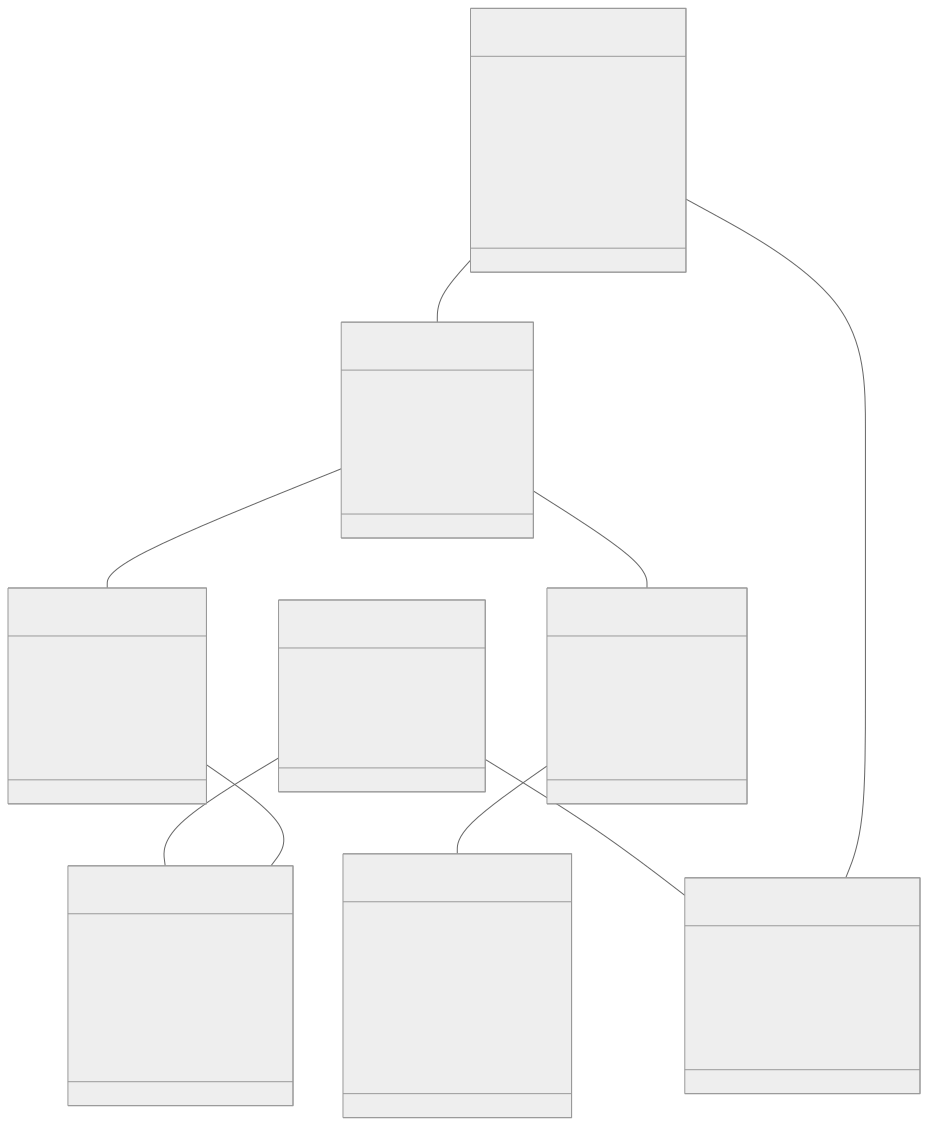
\includegraphics[width=0.9\textwidth]{component_relationships.png}
    \caption{Component Relationships}
\end{figure}

Key interactions between components include:
\begin{itemize}
    \item Frontend communicates exclusively through the API Gateway
    \item Lambda functions interact with databases and other AWS services
    \item Cognito handles all authentication before business logic executes
    \item Event-driven architecture connects components asynchronously where appropriate
\end{itemize}

\chapter{Data Models}

\section{Database Schema}
The database design incorporates relational, document, and graph capabilities through SurrealDB's multi-model approach.

\begin{figure}[ht]
    \centering
    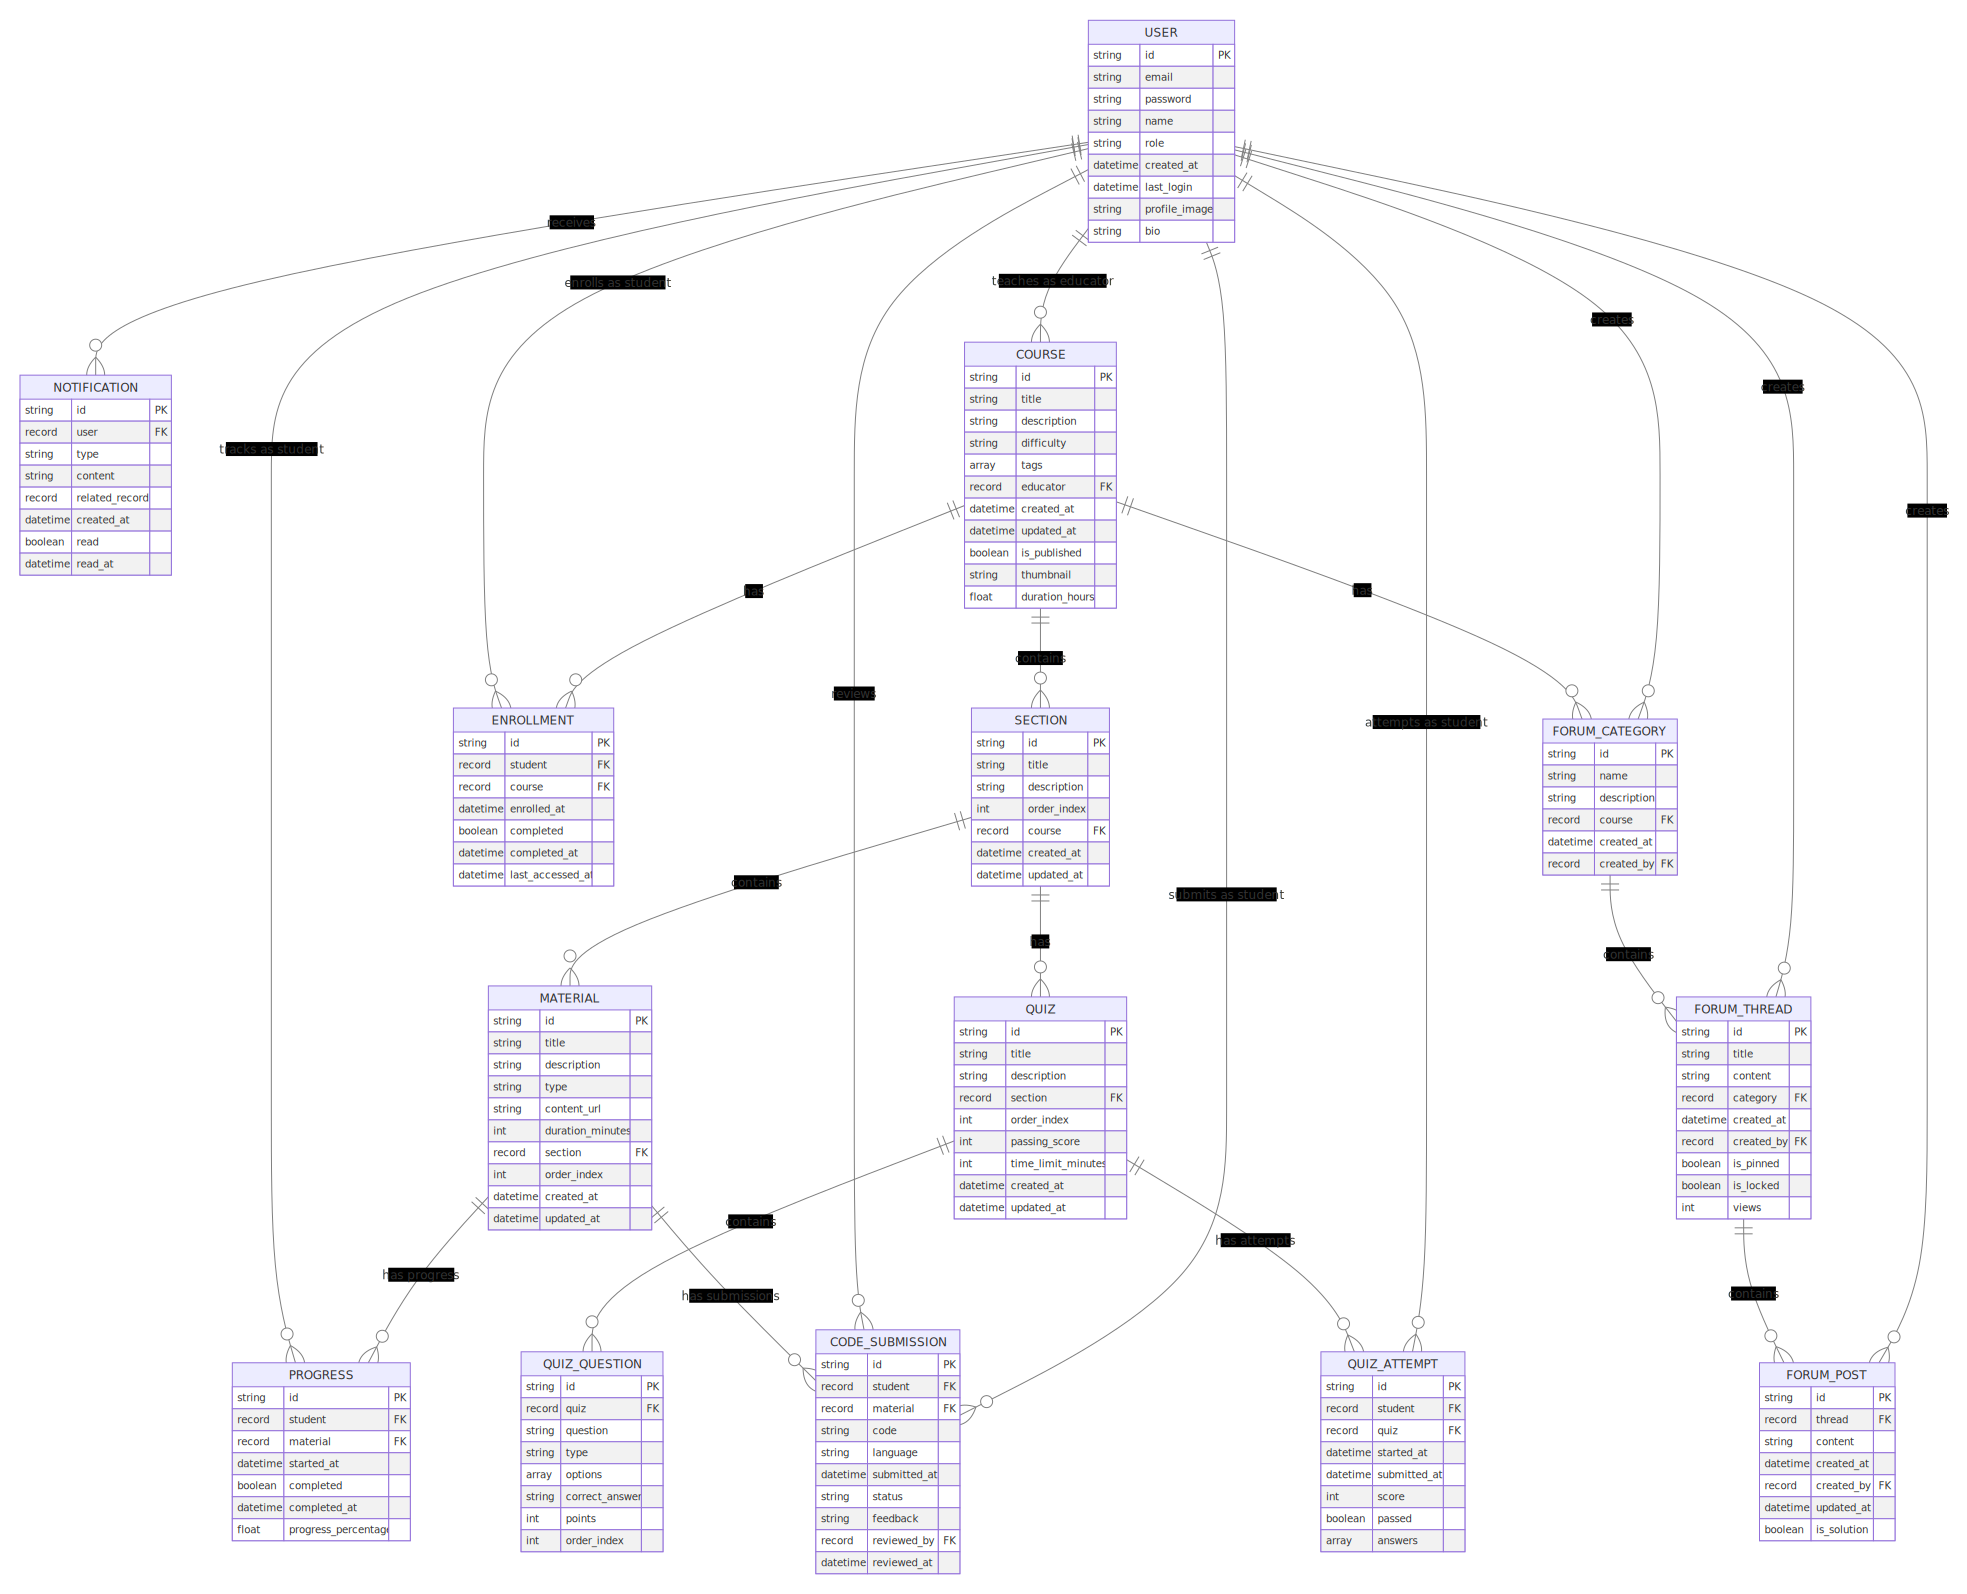
\includegraphics[width=0.9\textwidth]{database_schema.png}
    \caption{Database Schema}
\end{figure}

\section{Core Entities}
\begin{description}
    \item[User:] Contains user information, roles, and authentication details.
    \item[Course:] Represents a learning unit with metadata and organizational structure.
    \item[Section:] Organizational unit within courses containing materials.
    \item[Material:] Content items (videos, PDFs, code exercises) within sections.
    \item[Enrollment:] Maps relationships between users and courses.
    \item[Progress:] Tracks user advancement through materials.
    \item[Quiz/Assessment:] Contains questions and evaluation criteria.
    \item[Submission:] Stores user responses to assessments.
    \item[ForumPost:] User discussions and questions within the community.
\end{description}

\section{Data Flow}
The following diagram illustrates the flow of data through the system:

\begin{figure}[ht]
    \centering
    \includegraphics[width=0.9\textwidth]{data_flow.png}
    \caption{Data Flow Diagram}
\end{figure}

\section{Key Data Flows}

\subsection{User Registration and Authentication}
\begin{enumerate}
    \item User submits registration data through frontend
    \item API Gateway routes to Authentication Lambda
    \item Lambda creates user in Cognito and SurrealDB
    \item JWT token returned for authenticated session
\end{enumerate}

\subsection{Course Creation and Publishing}
\begin{enumerate}
    \item Educator creates course structure through UI
    \item Course metadata and structure stored in SurrealDB
    \item Materials uploaded to S3 with references stored in database
    \item Publishing workflow updates visibility and notifies subscribers
\end{enumerate}

\subsection{Code Assessment and Grading}
\begin{enumerate}
    \item Student submits code solution
    \item Code executed in isolated sandbox
    \item Results compared against test cases
    \item Grading results stored in database and displayed to student
    \item Progress records updated automatically
\end{enumerate}

\subsection{Forum Moderation}
\begin{enumerate}
    \item User creates or flags post
    \item Post stored in database with metadata
    \item Moderators review flagged content
    \item Moderation actions update content status and notify relevant users
\end{enumerate}

\chapter{Interface Design}

\section{API Structure}
The API follows RESTful principles organized into domain-specific endpoints. All external communication occurs through a standardized API Gateway.

\begin{figure}[ht]
    \centering
    % \includegraphics[width=0.9\textwidth]{api_domains.png}
    \caption{API Domains and Organization}
\end{figure}

\section{Authentication Protocol}
\begin{itemize}
    \item OAuth2 for third-party authentication (Google, GitHub)
    \item JWT tokens for session management and API authentication
    \item MFA via TOTP (Time-based One-Time Password) for sensitive operations
\end{itemize}

\section{Service Communication}

\subsection{External Interfaces}
\begin{itemize}
    \item RESTful APIs with JSON payloads
    \item Rate limiting (10 requests/second per user)
    \item Batch operations for efficiency
    \item Pagination for large result sets
\end{itemize}

\subsection{Internal Communication}
\begin{itemize}
    \item AWS SNS/SQS for asynchronous event processing
    \item AWS Step Functions for complex workflows
    \item Direct Lambda invocations for synchronous operations
\end{itemize}

\section{Error Handling}
\begin{itemize}
    \item Standardized error responses with HTTP status codes and descriptive messages
    \item Comprehensive logging with correlation IDs
    \item Global and resource-specific rate limiting
    \item Circuit breakers for downstream service failures
\end{itemize}

\section{Security Implementation}
\begin{figure}[ht]
    \centering
    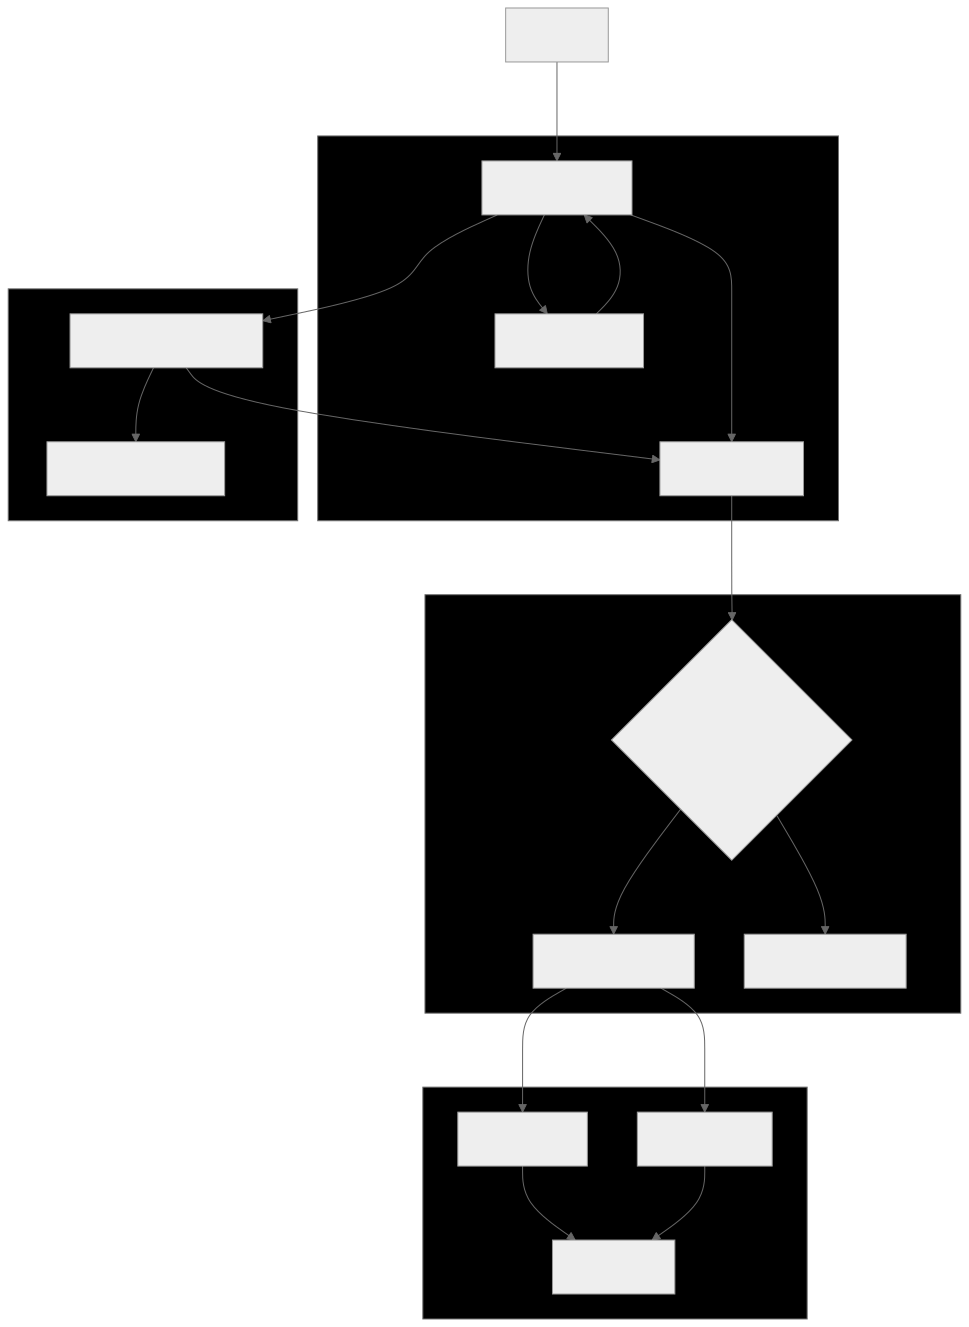
\includegraphics[width=0.9\textwidth]{security_implementation.png}
    \caption{Security Implementation Diagram}
\end{figure}

\subsection{Authentication and Authorization}
\begin{itemize}
    \item Multi-factor Authentication (MFA): Optional for all users, required for administrators
    \item OAuth2 Integration: Support for Google, GitHub, and Microsoft accounts
    \item Role-based Access Control (RBAC): Granular permissions based on user roles
    \item JWT for API Authentication: Secure, stateless authentication for API requests
\end{itemize}

\subsection{Data Protection}
\begin{itemize}
    \item Encryption at Rest: AES-256 encryption for all sensitive data
    \item Encryption in Transit: TLS 1.2+ for all network communications
    \item PII Protection: Minimized collection of personally identifiable information
    \item Data Retention Policies: Automated purging of unnecessary data
\end{itemize}

\chapter{Component Design}

\section{Frontend Components}

\subsection{Layout Components}
\begin{description}
    \item[Navbar] Top navigation component with:
    \begin{itemize}
        \item Logo and site navigation
        \item Search functionality
        \item Notification center
        \item User profile dropdown
    \end{itemize}
    
    \item[Sidebar] Navigation component with:
    \begin{itemize}
        \item Course navigation
        \item Quick links to user dashboard
        \item Role-specific menus
        \item Collapsible sections
    \end{itemize}
    
    \item[Footer] Bottom component with:
    \begin{itemize}
        \item Terms and privacy links
        \item Contact information
        \item Copyright notices
    \end{itemize}
\end{description}

\subsection{Page Components}
\begin{description}
    \item[Dashboard] Main user interface with:
    \begin{itemize}
        \item Welcome section with personalized greeting
        \item Statistics cards showing progress and achievements
        \item Visualization charts for activity and progress
        \item Upcoming deadlines and calendar
    \end{itemize}
    
    \item[Course Browser] Course discovery component with:
    \begin{itemize}
        \item Filterable/sortable course grid
        \item Category navigation
        \item Featured course carousel
        \item Course preview cards
    \end{itemize}
    
    \item[Code Editor] Interactive coding environment with:
    \begin{itemize}
        \item Syntax highlighting for multiple languages
        \item Resizable panels for instructions/tests
        \item Run/Submit controls
        \item Result visualization
    \end{itemize}
\end{description}

\section{Backend Components}

\subsection{Authentication Service}
\begin{description}
    \item[Responsibilities:]
    \begin{itemize}
        \item User registration and authentication
        \item Token generation and validation
        \item Role management and authorization
        \item MFA enrollment and verification
    \end{itemize}
    
    \item[Input/Output:]
    \begin{itemize}
        \item Input: User credentials, registration data
        \item Output: JWT tokens, user profile information
    \end{itemize}
    
    \item[Key Functions:]
    \begin{itemize}
        \item \texttt{register\_user(user\_data) -> Result<UserProfile, AuthError>}
        \item \texttt{authenticate\_user(credentials) -> Result<AuthToken, AuthError>}
        \item \texttt{validate\_token(token) -> Result<TokenClaims, AuthError>}
        \item \texttt{change\_user\_role(user\_id, role) -> Result<(), AuthError>}
    \end{itemize}
\end{description}

\subsection{Course Management Service}
\begin{description}
    \item[Responsibilities:]
    \begin{itemize}
        \item Course CRUD operations
        \item Content organization and delivery
        \item Enrollment management
        \item Progress tracking
    \end{itemize}
    
    \item[Input/Output:]
    \begin{itemize}
        \item Input: Course data, enrollment requests, content updates
        \item Output: Course structures, material access, progress reports
    \end{itemize}
    
    \item[Key Functions:]
    \begin{itemize}
        \item \texttt{create\_course(course\_data) -> Result<CourseId, CourseError>}
        \item \texttt{update\_course(course\_id, updates) -> Result<(), CourseError>}
        \item \texttt{enroll\_user(course\_id, user\_id) -> Result<Enrollment, EnrollmentError>}
        \item \texttt{update\_progress(user\_id, material\_id, progress) -> Result<Progress, ProgressError>}
    \end{itemize}
\end{description}

\subsection{Assessment Service}
\begin{description}
    \item[Responsibilities:]
    \begin{itemize}
        \item Quiz and assessment creation
        \item Code execution in sandboxed environment
        \item Automated grading
        \item Submission management
    \end{itemize}
    
    \item[Input/Output:]
    \begin{itemize}
        \item Input: Assessment definitions, code submissions, quiz responses
        \item Output: Execution results, grades, feedback
    \end{itemize}
    
    \item[Key Functions:]
    \begin{itemize}
        \item \texttt{create\_assessment(assessment\_data) -> Result<AssessmentId, AssessmentError>}
        \item \texttt{execute\_code(code, language, inputs) -> Result<ExecutionResult, ExecutionError>}
        \item \texttt{grade\_submission(submission) -> Result<Grade, GradingError>}
        \item \texttt{get\_submission\_history(user\_id, assessment\_id) -> Result<Vec<Submission>, SubmissionError>}
    \end{itemize}
\end{description}

\subsection{Forum Service}
\begin{description}
    \item[Responsibilities:]
    \begin{itemize}
        \item Discussion thread management
        \item Post moderation
        \item Content filtering
        \item Notification dispatching
    \end{itemize}
    
    \item[Input/Output:]
    \begin{itemize}
        \item Input: Forum posts, moderation actions, thread creation
        \item Output: Thread listings, post content, moderation results
    \end{itemize}
    
    \item[Key Functions:]
    \begin{itemize}
        \item \texttt{create\_post(post\_data) -> Result<PostId, ForumError>}
        \item \texttt{moderate\_post(post\_id, action) -> Result<(), ModerationError>}
        \item \texttt{get\_thread(thread\_id) -> Result<Thread, ForumError>}
        \item \texttt{get\_flagged\_posts() -> Result<Vec<FlaggedPost>, ForumError>}
    \end{itemize}
\end{description}

\subsection{Class Structure}
The following class diagram represents the core domain model:

\begin{figure}[ht]
    \centering
    \includegraphics[width=0.9\textwidth]{class_diagram.png}
    \caption{Class Diagram}
\end{figure}

\chapter{User Interface Design}

\section{Design Principles}
The UI design follows these core principles:
\begin{itemize}
    \item \textbf{Consistency:} Unified design language across all pages
    \item \textbf{Accessibility:} WCAG 2.1 AA compliance for all users
    \item \textbf{Responsiveness:} Optimal experience across devices (320px and up)
    \item \textbf{Progressive Enhancement:} Core functionality works without JavaScript
    \item \textbf{Feedback:} Clear indication of system status and actions
\end{itemize}

\section{Site Map and Navigation Flow}

\begin{figure}[ht]
    \centering
    % \includegraphics[width=0.9\textwidth]{sitemap.png}
    \caption{Site Map and Navigation Flow}
\end{figure}

\section{Interface Storyboards}

\subsection{Authentication Flow}
\begin{figure}[ht]
    \centering
    % \includegraphics[width=0.9\textwidth]{auth_flow.png}
    \caption{User Authentication Storyboard}
\end{figure}

\subsection{Course Enrollment and Participation}
\begin{figure}[ht]
    \centering
    % \includegraphics[width=0.9\textwidth]{course_flow.png}
    \caption{Course Enrollment and Learning Storyboard}
\end{figure}

\subsection{Assessment Completion}
\begin{figure}[ht]
    \centering
    % \includegraphics[width=0.9\textwidth]{assessment_flow.png}
    \caption{Assessment Completion Storyboard}
\end{figure}

\section{Accessibility Considerations}
\begin{itemize}
    \item \textbf{Keyboard Navigation:} Full functionality available without mouse
    \item \textbf{Screen Reader Support:} Proper ARIA labels and semantic HTML
    \item \textbf{Color Contrast:} WCAG AA (4.5:1) minimum contrast ratios
    \item \textbf{Text Resize:} Interface remains functional when text is enlarged 200\%
    \item \textbf{Motion Control:} Animations can be disabled via prefers-reduced-motion
    \item \textbf{Assistive Technology:} Regular testing with NVDA, JAWS, and VoiceOver
    \item \textbf{Alternative Text:} All images include descriptive alt text
\end{itemize}

\section{Responsive Design}
\begin{itemize}
    \item \textbf{Mobile First:} Designed primarily for mobile, then enhanced for larger screens
    \item \textbf{Breakpoints:} Key breakpoints at 480px, 768px, 1024px, and 1440px
    \item \textbf{Layout Adaptations:} 
    \begin{itemize}
        \item Single column layout on mobile
        \item Sidebar appears as overlay on small screens
        \item Multi-column layout on tablets and larger
        \item Expanded dashboard visualizations on desktop
    \end{itemize}
    \item \textbf{Touch Targets:} Minimum 44×44px for all interactive elements
\end{itemize}

\chapter{Assumptions}

\section{Technical Constraints}

\subsection{Hardware Constraints}
\begin{itemize}
    \item \textbf{Minimum Device Specifications:} Users require devices with:
    \begin{itemize}
        \item At least 4GB RAM for smooth performance
        \item Screen resolution of 320px width minimum
        \item Internet connection with 5 Mbps minimum bandwidth
    \end{itemize}
    
    \item \textbf{Server Environment:} Development and deployment assumes:
    \begin{itemize}
        \item AWS cloud infrastructure
        \item Serverless architecture with AWS Lambda
        \item No dedicated hardware requirements
        \item Horizontal scaling capabilities
    \end{itemize}
\end{itemize}

\subsection{Software Constraints}
\begin{itemize}
    \item \textbf{Browser Support:} Application designed for:
    \begin{itemize}
        \item Modern browsers (Chrome, Firefox, Safari, Edge - latest 2 versions)
        \item HTML5 and JavaScript required
        \item No Internet Explorer support
    \end{itemize}
    
    \item \textbf{Development Environment:}
    \begin{itemize}
        \item Standardized Docker containers for development
        \item Rust 1.58+ for backend development
        \item Node.js 16+ for frontend development
        \item AWS CDK for infrastructure definition
    \end{itemize}
    
    \item \textbf{Mobile Support:}
    \begin{itemize}
        \item Responsive web design (no native app initially)
        \item Mobile browser focused (iOS Safari, Android Chrome)
    \end{itemize}
\end{itemize}

\section{Operational Assumptions}

\subsection{Load and Performance}
\begin{itemize}
    \item Maximum concurrent users: 10,000
    \item Peak submission rate: 10,000 code submissions per minute
    \item Average session duration: 30 minutes
    \item 80/20 read/write ratio for database operations
    \item Code execution takes maximum 5 seconds per submission
\end{itemize}

\subsection{Development Process}
\begin{itemize}
    \item Agile methodology with 2-week sprints
    \item CI/CD pipeline with automated testing
    \item Feature branching development workflow
    \item Containerized development environments
    \item Terraform for infrastructure provisioning
\end{itemize}

\subsection{Maintenance and Support}
\begin{itemize}
    \item 99.9\% uptime requirement excluding planned maintenance
    \item Scheduled maintenance windows during off-peak hours
    \item Automated backups performed daily and retained for 30 days
    \item Customer support available during business hours
    \item Issue response time within 24 hours
\end{itemize}

\section{Dependencies}

\subsection{Third-Party Services}
\begin{itemize}
    \item Authentication via OAuth providers (Google, GitHub, Microsoft)
    \item Payment processing through Stripe
    \item Email delivery through Amazon SES
    \item CDN services through AWS CloudFront
    \item Media transcoding through AWS MediaConvert
\end{itemize}

\subsection{External Systems}
\begin{itemize}
    \item LMS integration via LTI standard
    \item External code repositories (GitHub, GitLab)
    \item Social media sharing APIs
    \item Analytics integrations (Google Analytics, Mixpanel)
\end{itemize}

\end{document} 